



\chapter{Implementação}
\label{implementacao}





Neste capítulo, são explicados os detalhes da implementação deste projeto, incluindo especificamente o projeto Django que inclui o sistema de informação com a aplicação web (frontend/backend) e API REST e também a aplicação mobile em Phonegap. Para além disso, é descrita a implementação da simulação em \textit{hardware} para o cenário descrito no capítulo anterior bem como o sistema de deteção de intrusos. 

Segundo o ciclo de vida de um software, estabelecido por \textit{Munish Kaur et al.}\cite{Saini2014} que analisámos na secção X.X, este capitulo irá incluir, em parte, a fase de \textit{designing} mas sobretudo a fase de \textit{coding}. 





\section{Sistema de informação}


Relativamente ao projeto Django, numa primeira fase procedeu-se à incorporação do \ac{SGBD} PostgreSQL através do psycopg2\footnote{http://initd.org/psycopg/docs/}. O psycopg2 consiste num adaptador entre o PostgreSQL com a linguagem de programação Python, que permite executar de formar eficiente qualquer \textit{script} em \ac{SQL}. É de notar que nesta fase inicial, encontram-se instalados algumas aplicações nativas do Django entre as quais, o  \texttt{django.contrib.auth} e  o \texttt{django.contrib.sessions}. Através delas é possivel verificar o total funcionamento da base de dados uma vez que permitem criar automática das tabelas associadas ao utilizadores, grupos, permissões e respetivos conteúdos, administração, sessões entres outros. Estas tabelas são fundamentais ao bom funcionamento do sistema uma vez que são consideradas no modelo de dados descrito na secção XX. 


Posteriormente, procedeu-se à criação dos diferentes \texttt{Models} conforme a nomenclatura apresentada nas tabelas X e X da secção XX. O excerto de código seguinte pretende ilustrar a criação do \texttt{Model} associado à tabela que representa a estrutura \acl{SM}, com o respetivo identificador e atributos.  Após a criação de cada \texttt{Models} procedeu-se à migração dos dados para o \ac{SGBD} onde era possível verificar que as tabelas tinham sido criadas, através da utilização da ferramenta gráfica pgAdmin III. De modo a testar a estrutura criada, procedeu-se à introdução de dados através da zona administrativa do Django (figura X). Através dos dados introduzidos e descrevendo um cenário realista foi possível validar a estrutura e proceder à implementação da aplicação web e criação da \ac{API} \ac{REST}. 




\begin{lstlisting}[
language=Python,
showspaces=false,
basicstyle=\ttfamily,
numbers=left,
numberstyle=\tiny,
commentstyle=\color{gray}
]
class SensorModule(models.Model):
	id = models.AutoField(primary_key=True)
	name = models.CharField(max_length=128)
	seding_time = models.IntegerField()
	status_sm = models.BooleanField(default=True)
	baterry_sm = models.IntegerField()
	localization_sm = models.CharField(max_length=128)
		
	def __str__(self):
		return "#"str(self.id) + " name_"+str(self.name)


\end{lstlisting}


\begin{figure}[!htb]
	\centering
	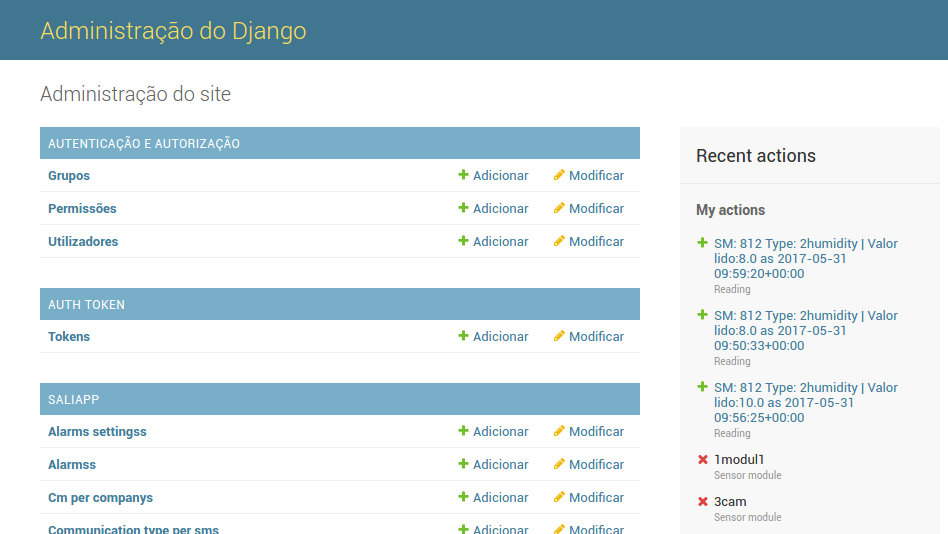
\includegraphics[scale=0.4]{prints-web/admindjango.png}
	\caption{Painel administrativo do Django }
	\label{activt-autent}
\end{figure}








\subsection{Sistema de registo e autenticação}

Primeiramente, procedeu-se à adaptação do template AdminLTE de modo a criar as páginas de autenticação e registo dos utilizadores. Como vimos anteriormente irão existir utilizadores distintos, uma vez que, de modo a identificá-los e a definir a sua permissões houve necessidade de criar grupos específicas. Foram então criados dois grupos:  \textit{company}, que identifica uma empresa e \textit{general}, que identificada um utilizador comum. O administrador do sistema é um utilizador que tem o estado de \textit{superuser} ativo, isto é, possui todas as permissões sem que estas lhe sejam atribuídas explicitamente.

\begin{figure}[!htb]
	\centering
	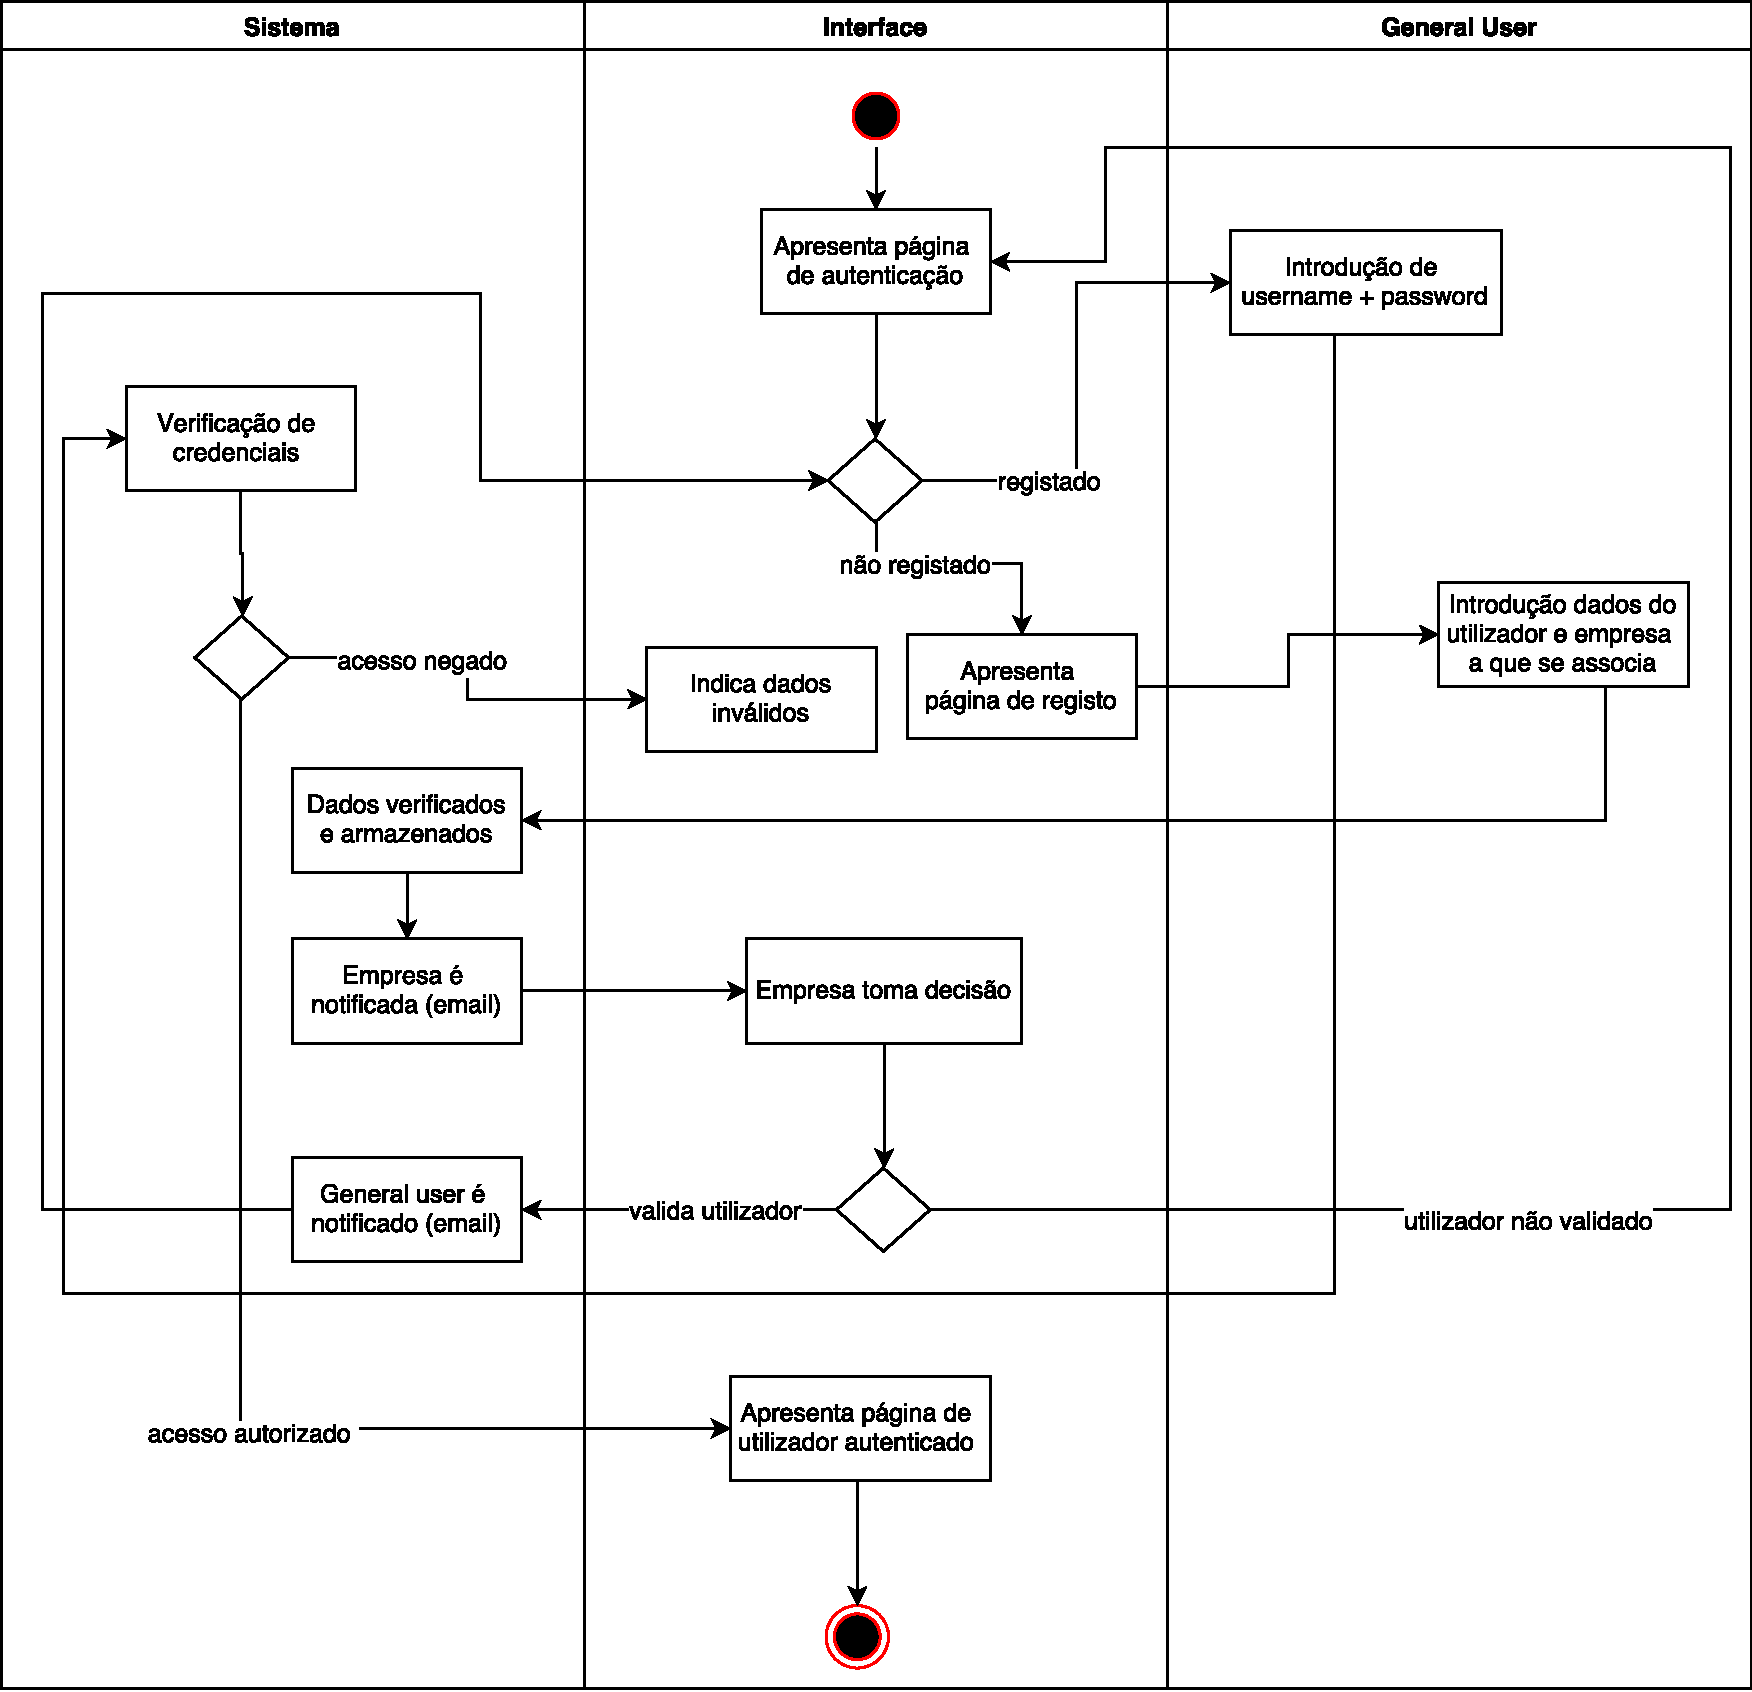
\includegraphics[width=\linewidth]{esquemas/activitydiagram-autenticacao.pdf}
	\caption{Diagrama de atividades do processo de registo e autenticação}
	\label{activt-autent}
\end{figure}



Como vimos anteriormente, o \textit{company user} apenas poderá ser adicionado ao sistema pelo admistrador, tendo este também permissões de gerir todos os utilizadores registados. Por outro lado, os \textit{company user} tem a possibilidade de validar os \textit{general user} que se associam à sua empresa, tendo posteriormente acesso aos dados/conteúdos da empresa. Após o registo de um novo \textit{general user} e validação por parte do \textit{company user}, existem notificações enviadas por email. Estas mensagens são enviadas recorrendo ao método \texttt{send\_mail()}\footnote{https://docs.djangoproject.com/en/1.11/topics/email/} existente nativamente no Django pelo pacote \texttt{django.core.mail}, sendo construido recorrendo ao módulo \texttt{smtplib}\footnote{Módulo que define objetos para sessões \ac{SMTP} https://docs.python.org/3/library/smtplib.html\#module-smtplib}. Na figura \ref{activt-autent} apresenta-se o diagrama de atividades que ilustra o processo de registo de um \textit{general user} que envolve o utilizador responsável pela empresa (company user). 







\subsection{Geração de alarmes}

No modelo de dados definido, cada sensor tem que ter obrigatoriamente associada uma tabela (AlarmsSettings) que permita definir o valor máximo e mínimo para o qual são gerados alarmes bem como as mensagens associadas para que o utilizador possa atuar.

 

 
cada sensor tem settings 

por cada leitura 
gerar alarmes
metodo verificação max min 
SQL 
stored procedure 
Trigger

forma mais eficaz: ??

\begin{figure}[!htb]
	\centering
	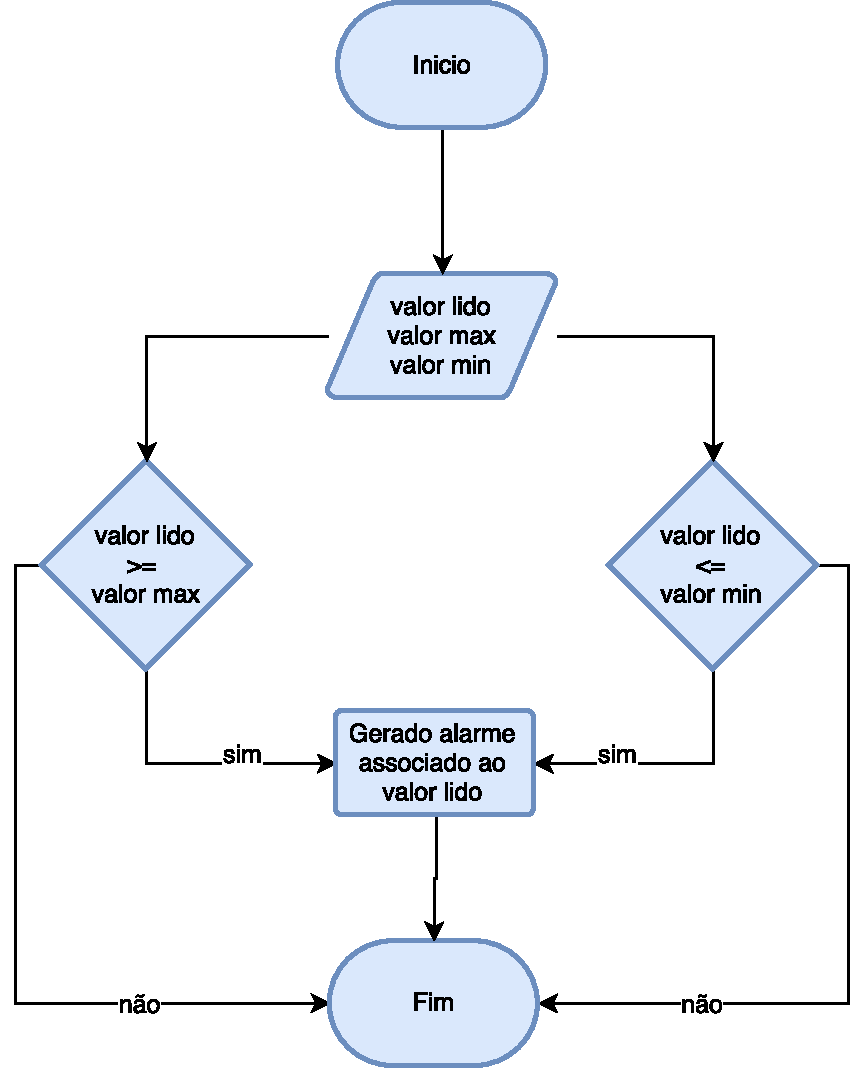
\includegraphics[scale=0.5]{esquemas/diagramafluxoalarms.pdf}
	\caption{Diagrama de fluxo para geração de alarmes}
	\label{activt-autent}
\end{figure}





\subsection{Visualização dos dados e cálculos estatísticos}





\subsection{\ac{API}}

tabela token 




\subsection{Documentação da \ac{API}}

\begin{figure}[h]
	\centering
	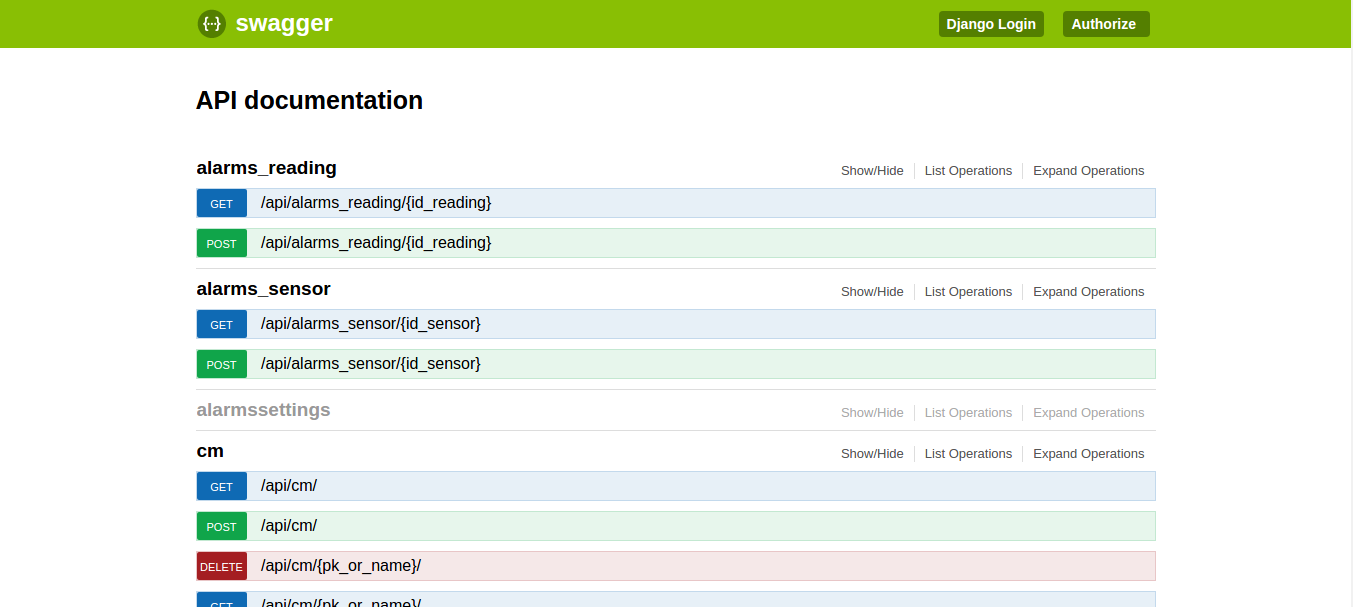
\includegraphics[width=\linewidth]{prints-web/api-doc.png}
	\caption{Arquitetura do sistema de informação (dashboard e API)}
	\label{docapi}
\end{figure}





\subsection{Aplicação web}

gravatar 

notificações https://docs.djangoproject.com/en/1.11/ref/contrib/messages/





\subsection{\textit{Deploy} do projecto}

\subsection{Aplicação mobile}


https://jee-appy.blogspot.com.tr/2015/04/deploy-django-project-on-apache-using.html

Caracteristicas da maquina virtual

Description:	Ubuntu 14.04.1 LTS
64 bitsRAM 2GB 


\begin{enumerate}
	\item Instalação da versão 2.7 python bem como pip e respectivo upgrade para a versão mais recente
	\item Instalação da versão xx do postgres e criação de uma base de dados com o nome salibd
	\item Instalação do apache2 e do mod\_wsgi que fará a ligação do projeto python com o servidor apache
	\item Instalação do virtualenv 
\end{enumerate}





\newpage
\section{Simulação em \textit{hardware}}

Nesta secção pretende-se explicar a implementação a nível de \textit{software} no contexto desta simulação para cada um dos micro-controladores. 


\subsection{Arduino}

No que diz respeito ao Arduino Nano (\ac{SM}), numa fase inicial,  procedeu-se à ligação dos diversos componentes anteriormente apresentados na \textit{breadboard} tal como se encontra apresentado no Anexo \ref{interlapd}. Para auxiliar o desenvolvimento de \textit{software} foi utilizada a versão 1.8.1 do \ac{IDE} do próprio Arduino\footnote{https://www.arduino.cc/en/Main/Software}.  

Seguidamente apresenta-se a implementação necessária a nível de sensores e de comunicação. 

\subsection{Sensores}



Foram desenvolvidos os seguintes métodos que permitem aceder aos valores lidos de cada um dos sensores. Para além disso, foi criado um método que permite alterar o estado do válvula para transferência de água. 

\begin{itemize}
	\item \texttt{int readTemperature(int port)}: é efetuada uma leitura no porto analógico. Após a leitura este é convertido para ºC (graus Celsius)
	
	\item \texttt{long readLuminosity(int port)}: 
	
	\item \texttt{int readWaterValve(int port)}: é efetuada uma leitura no porto digital através do método \texttt{digitalRead}. 
	
	\item \texttt{int readWaterLevel(int port)}: é efetuada uma leitura no porto digital através do método \texttt{digitalRead}.
	
	
	\item \texttt{void setWaterValve(int port, int state)}: se a variável \texttt{state} for 1 então o porto é colocado a \texttt{HIGH} (1) através do método \texttt{digitalWrite}, caso contrário é colocado a \texttt{LOW} (0)
	
\end{itemize}

Inicialmente procedeu-se à leitura de cada sensor de forma individual de modo a garantir o seu total funcionamento. Sempre que é feita um pedido de leitura dos sensores pelo \ac{CM} os valores são enviados com o seguinte formato: 

\begin{equation} 
\label{eq:someequation}
\texttt{<temperatura>;<nível\_água>;<luminosidade>;<estado\_válvula>}
\end{equation}

\subsection{Comunicação}


Numa primeira fase procedeu-se à comunicação entre o \ac{SM} e \ac{CM} através de porta série. Seguidamente resolveu-se incorporar o módulo bluetooth de modo a tornar cada módulo independente. De módulo de interagir com o módulo bluetooth utilizou-se o package \texttt{SoftwareSerial.h} disponível no Arduino. Decidiu-se que caso o módulo bluetooth recebesse valores de 0 a 2 tinha diferentes comportamentos: 

\begin{itemize}
	\item \textbf{0}: ativação (ligar) da válvula; 
	\item \textbf{1}: desativação (desligar) da válvula; 
	\item \textbf{2}: recebe dados obtidos pelos sensores no formato definido em (\ref{eq:someequation})
\end{itemize}

Antes de proceder à implementação de envio e receção de dados por bluetooth no Raspberry Pi 3 optou-se por testar este mecanismo através de uma aplicação Android existente na \textit{Play Store} chamada de \textit{Bluetooth Terminal HC-05}\footnote{https://play.google.com/store/apps/details?id=project.bluetoothterminal}

\subsubsection{Raspberry Pi}


\subsubsection{Comunicação}


Como é possível observar na figura \ref{esquemcomm}, para a comunicação no Raspberry Pi (\ac{CM}) entre o Arduino (\ac{SM}) foi utilizado o modulo interno de bluetooth 4.1 que este incorpora no seu hardware. Para tal, foi desenvolvido um \textit{script} em Python que permite o seguinte: 


\begin{enumerate}
	\item Verificar dispositivos bluetooth disponíveis
	\item Estabelecer conexão com módulo HC-06 através de um socket para comunicação utilizando para isso o \textit{package} \texttt{socket} do python. 
	\item Aceder à API para verificar estado da válvula de admissão de águas e enviá-lo através do socket utilizando o método \texttt{send()} 
	\item No caso se ser enviado o digito 1 a válvula será aberta, enquanto que se for enviado o digito 2 a válvula é fechada. 
	\item No caso de ser enviado o digito 2, o socket ficará à espera de receber os dados lidos pelos sensores, utilizando para isso o método \texttt{recv()}
	\item Após receber os dados lidos, é efetuado algum processamento para que os dados sejam enviados através da API. 
	\item Todos os pontos 3 a 6 são repetidos com um atraso igual ao seding time definido o sensor module na dashboard. 
	
\end{enumerate}

Para permitir o acesso aos recursos do sistema Bluetooth foi utilizada uma extensão (\textit{package}) do Python denominado de \textit{pybluez}\footnote{https://github.com/karulis/pybluez}. 




\subsection{Considerações finais}


>1 fase testar coneccao arduino to rasp via porta serie; foi criado um script em python para processar info e enviar para o servidor através da API 

>2 fase : necessidade de tornar um módulo isolado sem necessidade de fio; foi testado um modulo wifi e bluetooth; 

>neste contexto modulo wifi nao!... pretende-se que os sensor moduels sejam de baixo custo e low power. foi utilizado um modulo bluetooth; foi testada a conexao da comm bluetooth através de uma client disponveil na google play bluetooth terminal HC-05 


> 
pq nao foi usado um sensor de salinidade? nao havia orçamento.. 









\newpage
\section{Sistema de deteção de intrusos}





No que toca ao desenvolvimento, optou-se por utilizar o package picamera. Este pacote fornece  uma interface em Python (disponível para qualquer versão) para o módulo de câmara Raspberry Pi\footnote{http://picamera.readthedocs.io/en/release-1.13/}, permitindo uma fácil interação entre a aquisição da imagem e respetivo processamento. Neste contexto optou-se obviamente por utilizar a interface Python da biblioteca do OpenCV.



\subsection{Algoritmos de deteção de intrusos}
% artigo http://lear.inrialpes.fr/people/triggs/pubs/Dalal-cvpr05.pdf

De modo a estudar alguns algoritmos de deteção de pessoas foram estudados alguns artigos neste contexto. 


Para a resolução deste problema foi efetuados 


HOGDescriptor: classe que implementa um histograma de gradientes orientado ( [Dalal2005] ) detetor de objetos. 

hog = cv2.HOGDescriptor()
hog.setSVMDetector(cv2.HOGDescriptor\_getDefaultPeopleDetector())




Usado biblioteca do opencv que permite detectar 
HOGDescriptor


Deteção de intrusos: 

http://www.pyimagesearch.com/2015/11/09/pedestrian-detection-opencv/



versão simplificada: http://www.pyimagesearch.com/2015/02/16/faster-non-maximum-suppression-python/



Servidor em falsk 


deploy 
https://iotbytes.wordpress.com/python-flask-web-application-on-raspberry-pi-with-nginx-and-uwsgi/



Dataset: %http://www.robots.ox.ac.uk/ActiveVision/Research/Projects/2009bbenfold_headpose/project.html


é usado um detector HOG juntamente com um classificador linear SVM 





parametros do método detectMultiScale do opencv 

\begin{itemize}
	\item \texttt{img}: parâmetro obrigatório. 
	\item \texttt{hitThreshold}: parâmetro opcional. 
	\item \texttt{winStride}: parâmetro opcional. 
	\item \texttt{padding}: parâmetro opcional.  Os valores típicos para preenchimento incluem  (8, 8) ,  (16, 16) ,  (24, 24) , e  (32, 32) .
	
	
	\item \texttt{scale}: parâmetro opcional. 
	\item \texttt{finalThreshold}: parâmetro opcional. 
	\item \texttt{useMeanShiftGrouping}: parâmetro opcional. 
\end{itemize}





Neste contexto apenas foram utilizados os seguintes parâmetros winStride, scale, padding. 



\subsection{Testes}

Foram considerados 4 frames de imagens .... e no apêndice X




\subsection{Implementação}


%\subsection{Flask}

Flask é considerada uma microframework web desenvolvida em Python e baseado nas bibliotecas WSGI Werkzeug e Jinja2. Escolhi esta microframework pois pretende-se que esta seja executada num microcontrolador com baixos recursos. Para além disso, considera-se ser de fácil aprendizagem relativamente ao Django (já abordado na capitulo XX) e com uma ótima documentação. 




%\subsection{Servidor web NGNIX}

\section{Considerações finais}





